\documentclass[10pt,a4paper,titlepage]{article}
\usepackage[utf8]{inputenc}
\usepackage{amsmath}
\usepackage{amsfonts}
\usepackage{amssymb}
\usepackage{graphicx}
\author{Colter Radden-LeSage}
\title{Hill Climbing: Variations, Efficacy in Multidimentional Spaces, and Optimization}
\begin{document}

\maketitle
\section{Hill Climbing}

	Hill climbing is the basis for many optimization algorithms, but has limited usefulness due to the fact that it stops at the first local optimum that it finds.  This makes it well suited for searching relatively uninteresting search spaces. With the computing power of modern machines, searching spaces suited for hill climbing, even exhaustively, is somewhat trivial.
	
	Applying hill climbing to a very uneven search space yields unpredictable and erratic results because the optimum that hill climbing locates is very dependent on the location of the starting state.  This apparent weakness of hill climbing can be exploited if the approximate location of the global optimum in an uneven search space is known and the area surrounding the global optimum is smooth.
	
\begin{figure}[!ht]
  \centering
    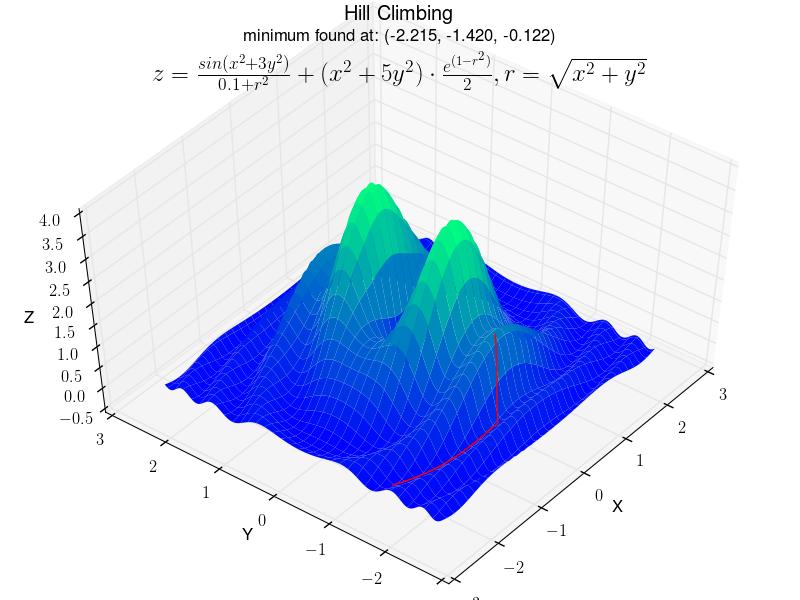
\includegraphics[width=\textwidth]{hill_climbing.png}
    \caption{Hill climbing finding local minimum in a search space with many local optima}
\end{figure}

\newpage
\section{Hill Climbing with Random Restarts}

Because the optimum found by hill climbing is somewhat predetermined by the starting position, a sensible way to overcome the barrier that irregular search spaces pose to hill climbing is by starting in many different positions within the space and tracking the best local optima that has been found.  Although this is an improvement from standard hill climbing, particularly "jagged" search spaces are still not well suited for hill climbing with restarts because finding the global optimum is dependent on the probability of randomly starting in the locale of the global optimum.

\begin{figure}[!ht]
  \centering
    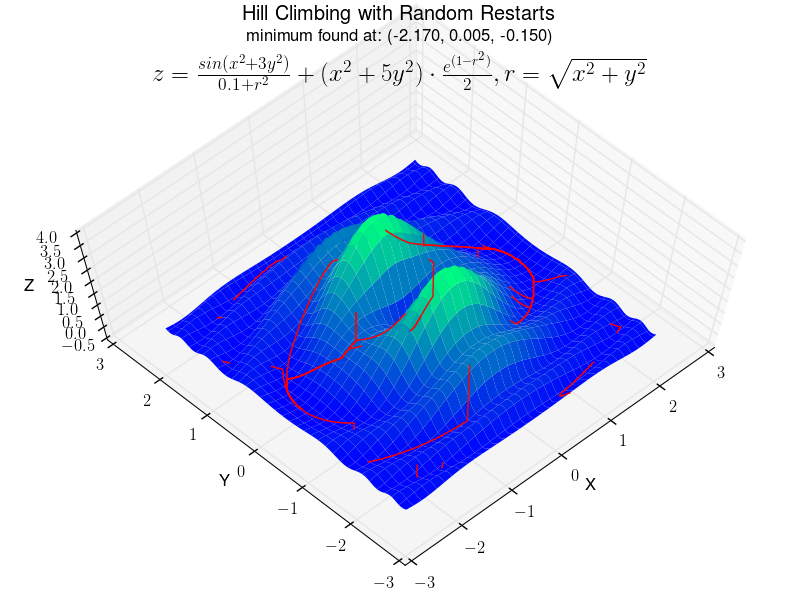
\includegraphics[width=\textwidth]{random_restarts.png}
    \caption{Locating global minima using hill climbing with random restarts}
\end{figure}

\newpage
\section{Simulated Annealing}

Simulated annealing is like hill climbing, but it has a probability of accepting a less-optimal state given by the formula:

\LARGE
\begin{center}
$P(S_a \rightarrow S_b) = e^\frac{f(S_a) - f(S_b)}{T}$
\end{center}

\normalsize
where $S_a$ is the current state, $S_b$ is some neighbouring state that is less optimal than $S_a$, $f(S)$ is the optimality function, and $T$ is the symbolic temperature of the system which is slowly lowered from a maximum value to zero.  Simulated annealing is better suited for locating global optima in uneven search spaces than traditional hill climbing or hill climbing with random restarts because simulated annealing is able to pass over local optima in search of the global optimum.

\begin{figure}[!ht]
  \centering
    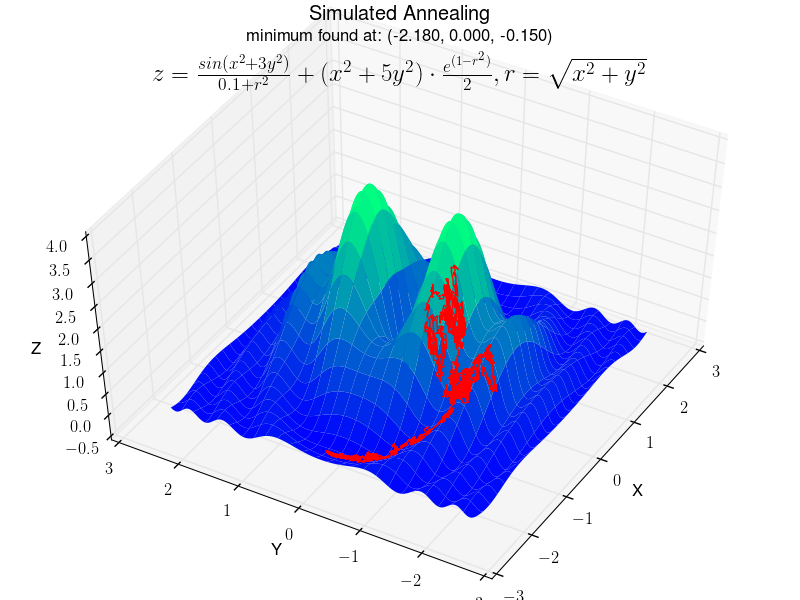
\includegraphics[width=\textwidth]{annealing_1.png}
    \caption{Simulated annealing searching less optimal states before locating the global minimum}
\end{figure}

\newpage
\section{Optimization of Simulated Annealing}
While implementing simulated annealing, it was discovered that many interconnected variables affect the ability of the algorithm to effectively find the global optimum.  Although simulated annealing can be generalized, it is recommended that its implementation be specific to the problem space being searched.

\subsection*{Maximum Temperature and Rate of Cooling}
One might assume that increasing the maximum temperature of the system would improve the outcomes of simulated annealing.  This change increases the number of cycles that simulated annealing runs, but improvements to the optimum returned by the algorithm are quickly diminishing.  This is because the equation describing the probability of accepting a worse state is dominated by $T$ while $T$ is high.  Increasing the maximum temperature prolongs the amount of time the algorithm is accepting worse states with a probability approaching 1 (good for overcoming large areas of poor states) and does nothing to increase the amount of time the algorithm spends effectively searching localities of the space.

The rate of cooling plays a far greater factor in the efficacy of simulated annealing.  The amount by which $T$ is lowered each cycle is what affects the number of cycles that the term $\frac{f(S_a) - f(S_b)}{T}$ is significant in the acceptance equation.  The major downside to choosing a lower constant cooling rate is that when a higher maximum temperature is necessary to overcome poor states in the search space, the additional cycles while $T$ is high are effectively redundant and needlessly extend the run time of the algorithm.

To create a balance between the need for a high maximum temperature and a low cooling rate, it is effective to express the cooling rate as the following function:

\LARGE
\begin{center}
$T_\Delta = \frac{T_{current}}{C \cdot T_{max}}$
\end{center}

\normalsize
where $T_\Delta$ is the cooling rate, $T_{current}$ is the current temperature, $T_{max}$ is the maximum temperature of the system, and $C$ is a positive constant.  Expressing the cooling rate as a function of the maximum temperature ensures that the majority of additional cycles that are added when $T_{max}$ is increased are carried out when $T_{current}$ is low (significant cycles) rather than when $T_{current}$ is high (cycles that only extend runtime).  This makes increasing $T_{max}$ more significant to the outcome of the algorithm without adding too many extraneous cycles.  A slight modification must be made to the standard simulated annealing algorithm to accommodate this optimization, though, because $T$ will approach 0 slowly but never actually reach 0.  The constant $C$ allows additional cycles to be added to the algorithm without affecting the value of $T$ in the acceptance function.

\newpage
\section{Analysis}
For the given function:
\LARGE
\begin{center}
$z = \frac{sin(x^2+3y^2)}{0.1+r^2}+(x^2+5y^2)\cdot\frac{e^{(1-r^2)}}{2},r=\sqrt{x^2+y^2}$
\end{center}
\normalsize
all three of the described search algorithms were applied.  Simulated annealing had the worst runtime of the three, using extra cycles to explore states that the algorithm knows are non-optimal.

The $z$ function is mirrored along both the $x$ and $y$ axes.  Therefore, searching the space from $(0, 0)$ to $(2.5, 2.5)$ yields one fourth of all possible combinations of $x$ and $y$ from $(-2.5, -2.5)$ to $(2.5, 2.5)$.  By dividing the domain from $(0, 0)$ to $(2.5, 2.5)$ into 10,000 combinations of $x$ and $y$ and applying basic hill climbing to all of those combinations, I have concluded that if the domain from $(-2.5, -2.5)$ to $(2.5, 2.5)$ were divided into 40,000 points, approximately 18,220 of all combinations of $x$ and $y$ can be followed using standard hill climbing to one of the global optima at $z=-0.150$.

The probability of randomly choosing a starting point that leads to the global optimum is therefore 45.55\% which is why basic hill climbing can find the global optimum nearly half the time.  Hill climbing with random restarts is therefore an excellent algorithm choice for this search space.  With a known probability of choosing a point that leads to the global optimum, calculating the minimum number of restarts, $n$, to reduce the probability of not finding the global optimum to $<$1\% is not difficult:

\begin{align*}
(1-0.4555)^n \leq 0.01
\\ log(0.5445^n) \leq log(0.01)
\\ n \cdot log(0.5445) \leq log(0.01)
\\ n \geq \frac{log(0.01)}{log(0.5445)}
\\ n \geq 7.58
\end{align*}

Therefore, with 8 restarts, hill climbing with random restarts will find the global optimum over 99\% of the time.


\end{document}